%!TEX root = CAN.tex
\section{Introduction}

The International Large Detector (ILD) \cite{ILC_TDR} considers a highly granular hadronic calorimeter using iron absorbers to achieve a compact detector with the best jet energy resolution around 3-4\% at 250 GeV satisfying the space constrain imposed by the solenoid magnet. Timing measurements in a calorimeter can be used to reject pile-up events like at the LHC or CLIC due to the bunch-to-bunch spacing of 25 and 0.5 ns respectively. Also the high level of $\gamma\gamma \rightarrow$ hadrons could be rejected by using timing information of the calorimeter in order to limit the impact of the background on physics measurements. Novel techniques of using time information to improve energy reconstruction could be used \cite{IEEE_timing}.\\
In the hadronic calorimeter, the timing precision is highly influenced by the time structure of the shower itself. A hadronic shower possesses several timing components related to different processes happening in the shower. A fast component related to instantaneous highly energetic deposits from high-energy hadrons and electromagnetic sub-showers. A slow component due to neutron scattering, nuclear-recoil and photons from nuclear processes, this component can last up to several milliseconds. Apart from physics processes, the measured hit time is influenced by the active medium used as well as the electronics. Time constants in the active medium such as scintillation decay time can affect the measurement.\\
The performance of the ILD relies on simulation studies based on \geant, it is important to study how well the simulation performs to reproduce the time structure of hadronic showers observed in data. The CALICE Analog Hadronic Calorimeter (AHCAL) technological prototype has been installed in the SPS CERN facilities in July and August 2015 in order to provide measurements using plastic scintillators. The goal of this study is to improve our knowledge about hadronic showers especially about its time evolution and time correlations of layers within the calorimeter. This note will describe the timing calibration procedure of the AHCAL first, the comparison with simulation for muons and electrons and finally a comparison with pion data.

\section{The CERN 2015 Testbeam Setup}

The datasets used in this note were collected during the testbeam campaign at CERN Super Proton Synchrotron (SPS) in July 2015. The SPS beamline provides secondary beams of hadrons, electrons and muons in a wide particle momenta range from 10 to 360 GeV/c. More details on the beamline are available in \cite{SPSBeamLine}.

\subsection{The CALICE AHCAL technological prototype}

In the July 2015 testbeam period, the CALICE AHCAL technological prototype setup consisted of 38 steel absorber plates, 17.2 mm thick, corresponding to a depth of approximately 40 $X_0$ ($\sim$ 4.5 nuclear interaction length $\lambda_{n}$). The active layers consisted of a iron cassette, 1 mm thick, a HCAL Base Unit (HBU) of an area of $36\times36$ cm$^2$, hosting the integrated readout electronics and a $30\times30\times3$ mm$^3$ plastic scintillator tile wrapped in a reflective foil. Each plastic tile is read out individually by a SiPM. The layers consisted of either 1 or 4 HBUs as illustrated in figure \ref{fig:detector_layout}.

\begin{figure}[htbp]
	\subfigure[%Picture of the AHCAL steel stack during the CERN testbeam.
	\label{fig:stack_steel}] {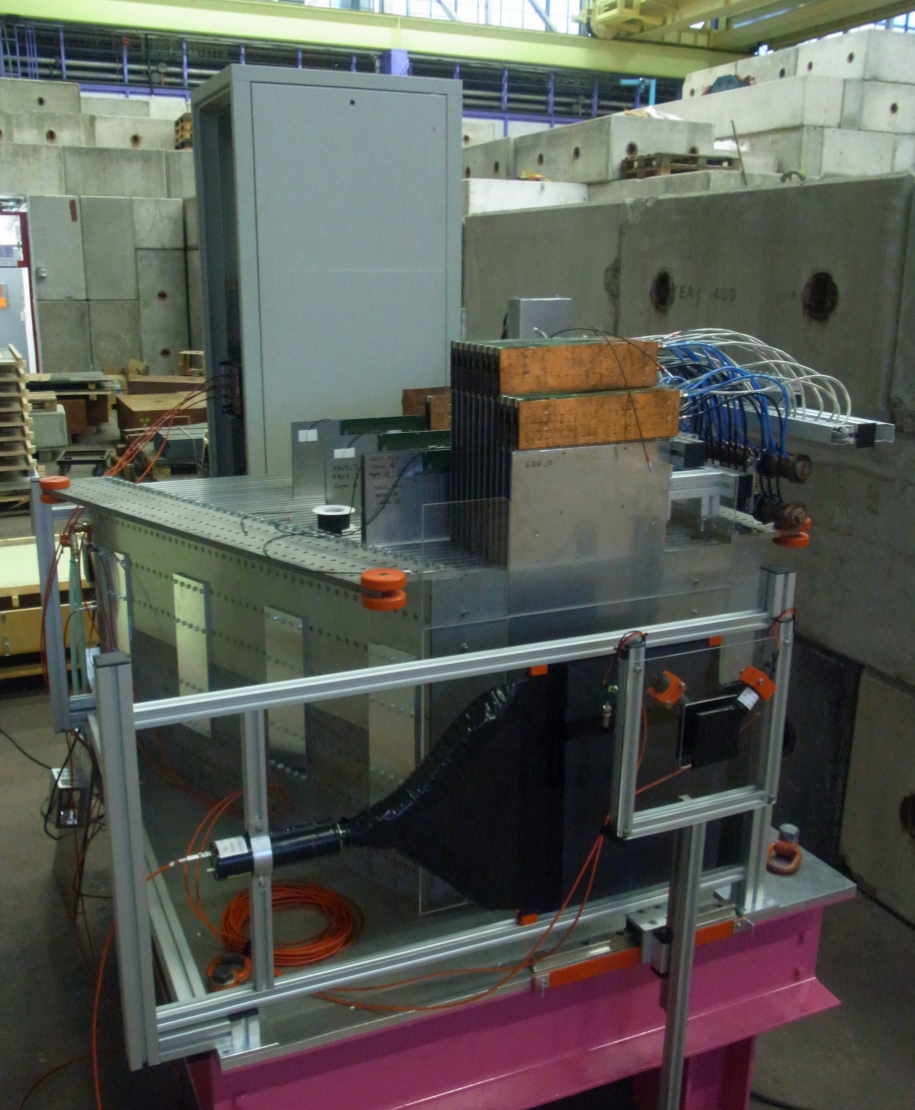
\includegraphics[width=0.35\textwidth]{fig/Others/steel_stack_ps.png}}\hfill
	\subfigure[%Detector layout of the CALICE AHCAL during the 2015 July Testbeam at the SPS.
	\label{fig:detector_layout}] {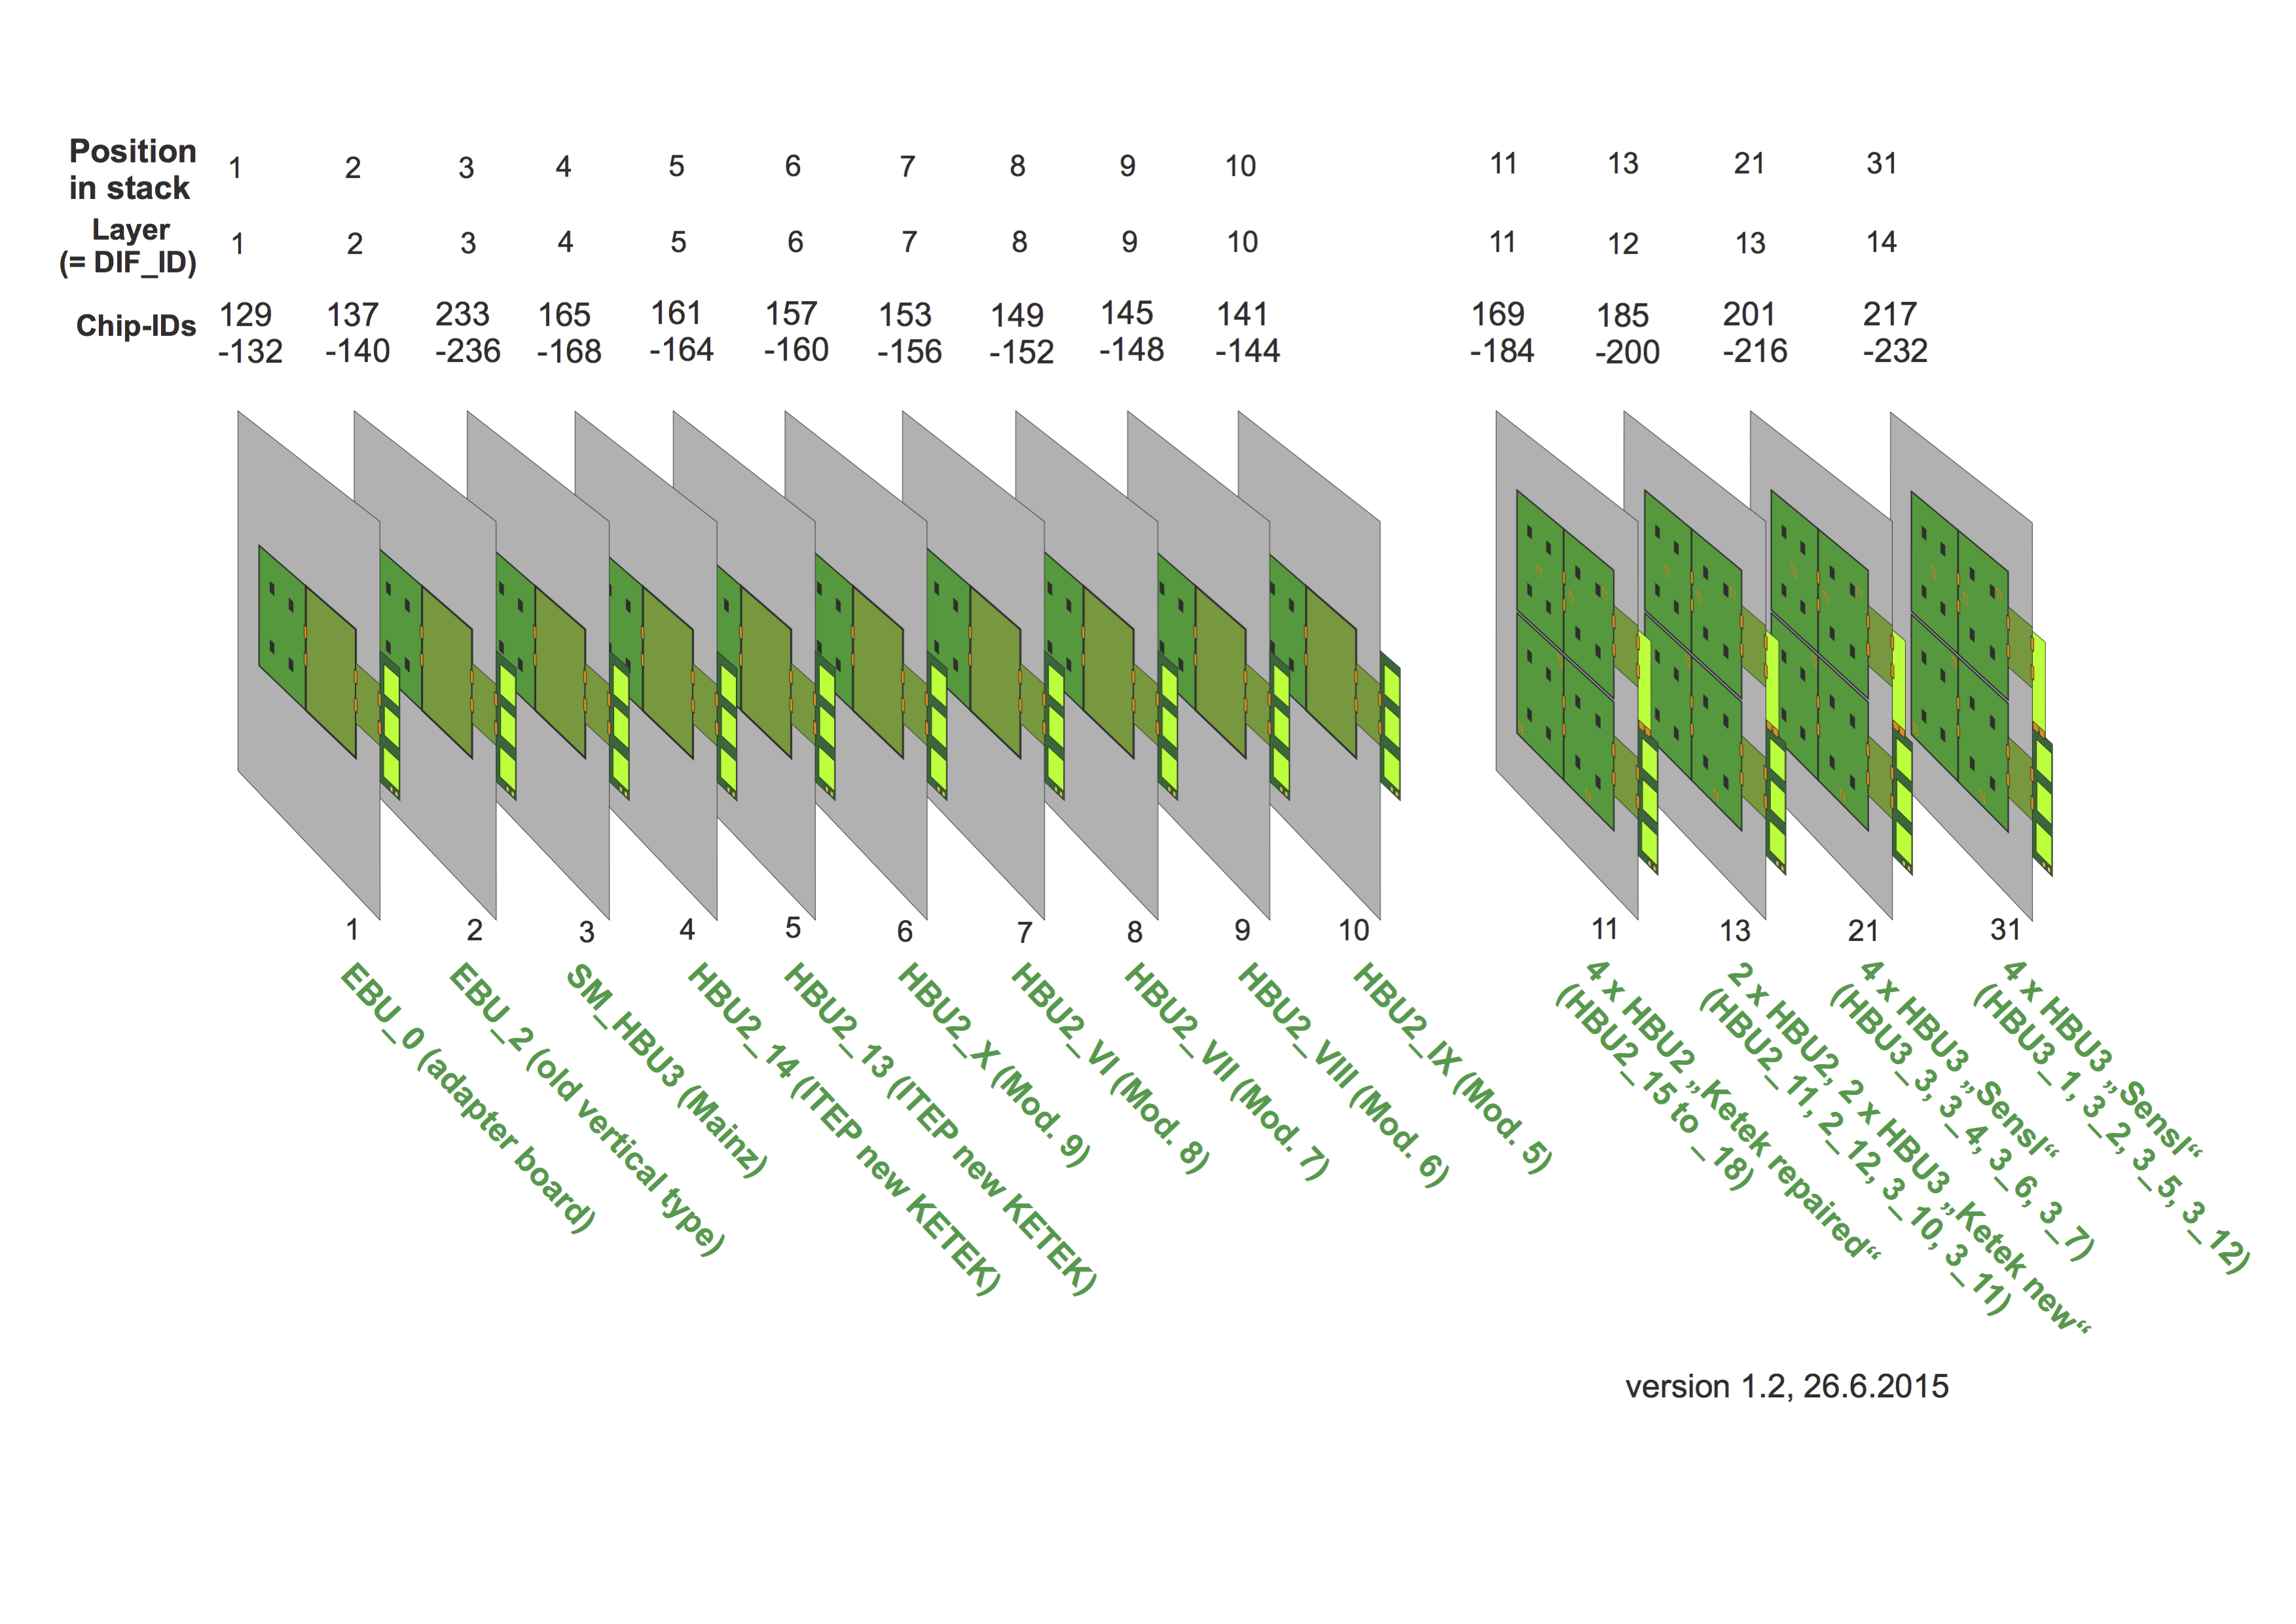
\includegraphics[width=0.60\textwidth]{fig/Others/Detector_layout.png}}
	\caption[]{\textbf{a}: Picture of the CALICE AHCAL during the Testbeam in July 2015 at CERN. The trigger scintillators can be seen in front of the stack in the photo. \textbf{b}: Layout used during the July 2015 SPS Testbeam campaign.}
	\label{fig:full_detector_layout}
\end{figure}

\subsection{Testbeam Setup}

The two first layers consisted of ECAL Base Unit (EBU) with 144 scintillator strips of $45\times5\times2$ mm$^3$ read out by SiPMs for a total area of $18\times18$ cm$^2$. The next 8 layers consisted of a single HBU that can be used as a shower start finder in order to locate the first hard hadronic interaction. And the last 4 layers consisted of $2\times2$ HBUs in order to study timing of hadronic showers. The prototype was equipped by various SiPM types and tile designs that are summed up in table \ref{table:sipm_list}. The total number of channels is of 3744.
\begin{table}[h!]
\centering
\resizebox{\textwidth}{!}{%
	\begin{tabular}{cccccccc}
	\hline
    Layer\# & Producer & Model & Area (mm$^2$) & Pitch ($\mu$m) & WLS Fibre & Read out & Slot\\
    \hline
    1 & Hamamatsu & S12571\_010P & $1\times1$ & 10 & no & Bottom & 1\\
    2 & Hamamatsu & S10362-11-025O & $1\times1$ & 25 & no & Side & 2\\
    3 & Hamamatsu & S12571-025P & $1\times1$ & 25 & no & SMD & 3\\
    4-5 & Ketek & N/A & $2.25\times2.25$ & 18 & no & Side & 4-5\\
    6-10 & CPTA & CPTA & $1.28\times1.28$ & 40 & yes & Side & 6-10\\
    11-12 & Ketek & PM1125NS-SB0 & $1.2\times1.2$ & 25 & no & Side & 11-13\\
    13-14 & SenSL & MicroFB-10020-SMT & $1\times1$ & 20 & no & Side & 21-31\\
    \hline
    \end{tabular}
    }
\caption{List of the different SiPMs used in the CALICE AHCAL in July 2015.}
\label{table:sipm_list}
\end{table}

\subsection{The SPIROC2b chip}

The SiPMs are read out by a SPIROC2b chip which features 36 channels measuring ADC amplitudes (energy) and TDC amplitudes (time) and can store up to 16 events. The collected charge from the SiPM is stored in a capacitor (memory-cell) waiting to be digitised with a 12 bit range. The chip can be configured in 2 different modes. An external trigger mode is used for gain calibration via an integrated LED Calibration System and monitoring of the SiPM gain. An auto-trigger mode is used to collect physics data. A threshold between 0.2-0.5 MIP is set for each chip in the setup. The SiPM signal is amplified by a pre-amplifier with two different gains (High Gain and Low Gain) and then is integrated by a slow shaper (50 ns shaping time) before being stored into a memory cell. The time is measured via a fast shaper (15 ns shaping time) integrating the signal. When the signal passes the threshold and it is measured by a voltage ramp (TDC ramp). Each chip possesses two voltage ramps that are multiplexed when a new Bunch Crossing (BXID) occurs. The length of a BXID is defined by the slow clock of the chip. In testbeam, the clock used is of 250 kHz which would correspond to a BXID length of 4 $\mu$s but due to the ramp multiplexer a dead time of around 2\% has to be taken into account. Thus the ramp length is 3.92 $\mu$s \cite{EldwanSSP}. For testbeam operation, a validation signal coming from scintillator beam triggers can be provided to the chip in order to suppress noise hits \cite{DAQ}.\\
\begin{figure}[htbp]
\begin{center}
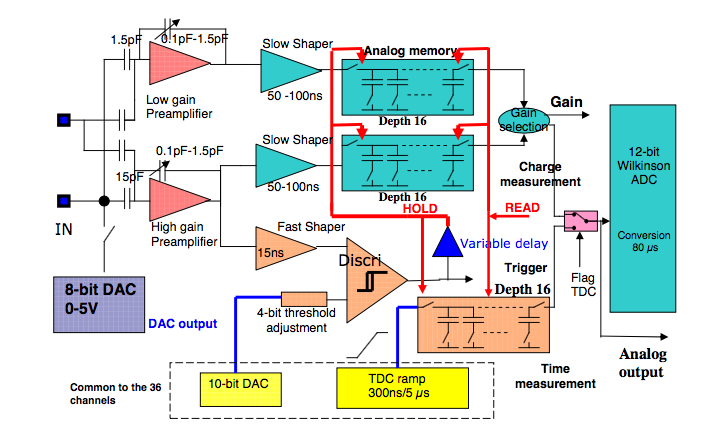
\includegraphics[width=0.7\textwidth]{fig/Others/Spiroc_layout.png}
\caption{Schematic of the signal path of the SPIROC2B for a single channel \cite{SPIROCManual}.}
\label{fig:SPIROC2B}
\end{center}
\end{figure}

\subsection{Trigger Signals}
\label{subsec:trigger}

For a muon beam, two scintillator plates of $50\times50$ cm$^2$ were placed in front and back of the calorimeter. For electron and pion beams, two small scintillator plates of $10\times10$ cm$^2$ were positioned in front of the calorimeter (see figure \ref{fig:stack_steel}). The trigger scintillators were connected to a NIM-logic (discriminator and gate) in order to provide a validation of the data to the chip.
In order to provide the time reference of the triggers, a SiPM-like pulse of around 4 $\mu$s length and with a fast rising edge around 1 ns was generated from the NIM-logic. This signal was injected directly via AC coupling to some channels in the setup as shown in the table \ref{table:trigger_signal_list}. No other external time reference than these channels is available.
\begin{table}[htbp]
\centering
  \begin{tabular}{@{} ccccc @{}}
    \hline
    Layer \# & Chip Number & Channel & Comments & Appellation \\
    \hline
    11 & 169 & 29 & noisy & T$_{11}$ \\
    11 & 177 & 23 & broken & - \\
    12 & 185 & 29 & - & T$_{12}$ \\
    13 & 201 & 29 & -  & T$_{13}$ \\
    13 & 211 & 6 & broken & - \\
    14 & 217 & 23 & - & T$_{14}$ \\
    \hline
  \end{tabular}
  \caption{List of channels with the injected trigger signal to be used as time reference.}
  \label{table:trigger_signal_list}
\end{table}
In the following analysis, only the reference signals T$_{12}$,  T$_{13}$ and T$_{14}$ were used.

\section{Runs \& Event Selection}

\subsection{Dataset}
\label{subsec:dataset}
During the campaign at SPS in July 2015, $\mu^-$ runs were taken at 50 and 150 GeV beam energy for the calibration of the detector. Several e$^{-}$ runs were taken between 10 to 50 GeV beam energy to study the electromagnetic response of the calorimeter. The e$^{-}$ runs were quite pure as the beam was generated via a neutral beam directed on a converter target. Due to the significant amount of air and beam line instrumentation between the calorimeter and the final momentum selection magnet as well as few information of the beam parameters, the beam profile of electron runs is not well reproduced in simulation. Finally, $\pi^-$ runs were taken between 10 to 90 GeV beam energy. The table \ref{table:dataruns} sums up the dataset taken.
\begin{table}[htbp]
\centering
\resizebox{0.8\textwidth}{!}{%
  \begin{tabular}{@{}l||p{2cm}p{8cm}@{}}
    \hline
    \multicolumn{1}{l}{\textbf{Particle}} & \textbf{Energy} & \textbf{Runs}\\
    \hline
    \multirow{2}{*}{$\mu^-$}& 50 GeV & 24016-24204\\& 150 GeV & 24623-24662\\
    \hline
    \multirow{2}{*}{e$^-$}& 10 GeV & 24531-24576\\& 15 GeV & 24507-24527\\& 20 GeV & 24479-24504\\& 30 GeV & 24454-24475\\& 40 GeV & 24420-24448\\& 50 GeV & 24404-24419\\
    \hline
    \multirow{2}{*}{$\pi^-$}& 10 GeV & 24266-24272, 24300-24317, 24381-24397\\& 20 GeV & 24398-24400\\& 30 GeV & 24259-24299, 24319-24380\\& 50 GeV & 24212-24254, 24325-24357, 24580-24612\\& 70 GeV & 24219-24242, 24365-24374\\& 90 GeV & 24233-24287, 24331-24364\\
    \hline
    \end{tabular}
    }
  \caption{List of runs taken at SPS in July 2015.}
  \label{table:dataruns}
\end{table}
\subsection{Muon Selection}
The $\mu$ runs were taken first at 50 GeV then another scan at the end of the campaign was performed at 150 GeV. The muon beam was produced by scrapping the halo of a secondary pion beam using collimators. The muon runs were contaminated by pions, a first estimation provided that around 30\% of the events were contaminated. The main goal of the muon selection was to efficiently select muons and reject pion showers. For this, a simple track finder has been developed. In order to select muons or punch-through pions, a straight track of at least 7 hits is required in the whole AHCAL without a hard interaction. In addition to reject late pion showers, not more than 2 hits are required per layer.
\begin{table}[htbp]
\centering
\resizebox{0.9\textwidth}{!}{%
  \begin{tabular}{@{}p{4cm} p{3cm} p{6cm}@{}}
    \hline
    \multicolumn{1}{l}{\textbf{Name}} & \textbf{Beam Energy} & \textbf{Cut}\\
    \hline
    \multirow{2}{*}{Preselection}& All & 0 mm < $cog_{z}$ < 800 mm\\& All & 0 < $n_{hits}$ < 20 \\
    \hline
    \multirow{2}{*}{Track Selection SSF}& All & $n_{hits}$ in tower > 7 \\& All & $n_{hits}$ in layer < 3 \\
    \hline
    \multirow{2}{*}{Track Selection BL}& All & $n_{hits}$ in tower > 2 \\& All & $n_{hits}$ in layer < 3 \\
    \hline
    \end{tabular}
    }
  \caption{Selection cuts for muon runs.}
  \label{table:muon_sel}
\end{table}
\subsection{Electron Selection}
\label{subsec:elec_sel}
To perform comparisons on electron, a sample of events is selected from the data runs. A simple selection is performed in order to have mostly contained showers in the AHCAL. The selection cuts are summed up in table \ref{table:electron_sel} for each energies.
\begin{table}[htbp]
\centering
\resizebox{0.9\textwidth}{!}{%
  \begin{tabular}{@{}p{4cm} p{3cm} p{6cm}@{}}
    \hline
    \multicolumn{1}{l}{\textbf{Name}} & \textbf{Beam Energy} & \textbf{Cut}\\
    \hline
    \multirow{2}{*}{Event Quality}& All & Cherenkow ON\\& All & Energy in the first 3 layers of AHCAL > 10 MIP \\
    \hline
    \multirow{9}{*}{Electron Selection}& 10 GeV & 25 < $n_{hits}$ < 75 \\& 15 GeV & 30 < $n_{hits}$ < 90 \\& 20 GeV & 40 < $n_{hits}$ < 100 \\& 30 GeV & 50 < $n_{hits}$ < 110 \\& 40 GeV & 60 < $n_{hits}$ < 120 \\& 50 GeV & 70 < $n_{hits}$ < 140 \\& All & $cog_{z}$ < 250 mm\\& All & -90 mm < $cog_{x, y}$ < 90 mm \\& All & Energy in last two layers < 1\% $E_{sum}$ \\
    \hline
    \end{tabular}
    }
  \caption{Selection cuts for each electron energies.}
  \label{table:electron_sel}
\end{table}
\subsection{Pion Selection}
A simple selection is performed on pion events. The goal is to reject punch-through pions, muons and electron contamination. The selection cuts are shown in table \ref{table:pion_sel}.
\begin{table}[htbp]
\centering
\resizebox{0.9\textwidth}{!}{%
  \begin{tabular}{@{}p{4cm} p{3cm} p{6cm}@{}}
    \hline
    \multicolumn{1}{l}{\textbf{Name}} & \textbf{Beam Energy} & \textbf{Cut}\\
    \hline
    \multirow{1}{*}{Event Quality}& All & Cherenkow OFF\\
    \hline
    \multirow{3}{*}{Pion Selection}& All & $n_{hits}$ > 20 \\& All & $n_{hits}$ in the first 2 AHCAL layers < 5 \\& All & Energy in last two layers > 1\% $E_{sum}$ \\
    \hline
    \end{tabular}
    }
  \caption{Selection cuts for pions.}
  \label{table:pion_sel}
\end{table}
\section{Simulation}

\subsection{AHCAL Simulation Model \& Digitisation}

The simulation of the testbeam prototype is based on the \mokka framework v08-05-01 and the new \ddhep framework v00-16, which both provide a full \geant v10-1 based simulation of the detector implementations with detailed geometry and material descriptions. The right handed coordinate is used such as the Z-axis points in the beam direction and that the Y-axis is directed upwards. No beamline instrumentation is simulated except scintillator triggers in front and back of the detector. An additional layer of 5.6 mm of lead is added in front of the calorimeter in order to account for missing upstream material. This analysis uses the sub-detector \mokka models \textit{TBecal4d} for the ScECAL (Scintillator strips with EBUs) and \textit{TBhcal4d} for the AHCAL. The distance between the sub-detectors is set to 0 mm. A check was performed between \mokka and \ddhep models with electrons and pions to ensure that the material description in both models are approximately the same.\\
The beam gun is placed 1 m in front of the calorimeter face for the simulations in this analysis. It is configured to generate single beam particle with a 2\% momentum spread (according to the beamline) and the beam profile for electrons and pions is extracted from data and applied to simulation. For muon runs, a flat beam covering the full AHCAL is simulated as this is not expected to have an influence on the MIP and time response of the detector.
All electron simulations are simulated with \geant 10.1 using the QGSP\_BERT\_HP physics list.\\
Pion showers are simulated using QGSP\_BERT, QGSP\_BERT\_HP and FTFP\_BERT\_HP physics lists as theses physics lists are well validated for the simulation of high energy showers in steel-scintillator sandwich calorimeter \cite{AHCAL_Physics}. The package \textit{high precision} (\_HP) is used in order to understand the differences induced in timing with a precise treatment of the neutrons.
For each energies, 100 000 simulated $\mu^-$, $e^-$ and 200000 $\pi^-$ single particle events are generated.\\
The digitisation of simulated hits is very similar to the one used in the ScECAL and AHCAL physics prototypes \cite{CAN-002, CAN-010, JINST-6}. Using, if available, individual calibration factors obtained from data to extract the light yield which is needed to model the statistical fluctuations of photons hitting a SiPM. Saturation effects are also included using the number of pixels available on each SiPM type. Most of the tiles used are wrapped with a reflective foil in order that crosstalk effect between channels can be neglected. For layers with no wrapping a default value of 15\% cross-talk is applied. The timing is modelled in the same way as in the SPIROC, the energy from sub-hits in a cell is integrated over a sliding time window of 15 ns, if the energy sum passes the threshold the time of the simulated sub-hit passing the threshold is registered as the time of the hit. In order to simulate detector resolution effects, the time of a hit is smeared with a double gaussian function with slightly different means and sigmas convoluted with a gaussian of fixed mean and variable sigma. More details are explained in appendix \ref{appendix:ped_shift}. Noise needs to be taken into account for with the engineering AHCAL prototype. Noise is added using muon runs by removing found tracks and keeping remaining hits. This is described in appendix \ref{appendix:noise}.\\
After digitisation, simulated hits have the same format as raw data hits and are then reconstructed using the same software chain used for data. To suppress noise, only hits above 0.5 MIP are considered in this analysis in both simulation and data.
